%
% LaTeX template for prepartion of submissions to PLDI'16
%
% Requires temporary version of sigplanconf style file provided on
% PLDI'16 web site.
% 
\documentclass[pldi]{sigplanconf-pldi16}
% \documentclass[pldi-cameraready]{sigplanconf-pldi16}

%
% the following standard packages may be helpful, but are not required
%
\usepackage{SIunits}            % typset units correctly
\usepackage{courier}            % standard fixed width font
\usepackage[scaled]{helvet} % see www.ctan.org/get/macros/latex/required/psnfss/psnfss2e.pdf
\usepackage{url}                  % format URLs
\usepackage{listings}          % format code
\usepackage{enumitem}      % adjust spacing in enums
\usepackage[colorlinks=true,allcolors=blue,breaklinks,draft=false]{hyperref}   % hyperlinks, including DOIs and URLs in bibliography
% known bug: http://tex.stackexchange.com/questions/1522/pdfendlink-ended-up-in-different-nesting-level-than-pdfstartlink
\newcommand{\doi}[1]{doi:~\href{http://dx.doi.org/#1}{\Hurl{#1}}}   % print a hyperlinked DOI


\usepackage[usenames,dvipsnames]{color}
\newcommand{\ruzica}[1]{\textcolor{Magenta}{\textsf{RP}: #1}}
\newcommand{\markk}[1]{\textcolor{Blue}{\textsf{MS}: #1}}
\newcommand{\alex}[1]{\textcolor{Orange}{\textsf{AR}: #1}}
\newcommand{\marvin}[1]{\textcolor{Green}{\textsf{MQ}: #1}}


\usepackage{comment}

\usepackage{graphicx}

\definecolor{identifierColor}{rgb}{0.65,0.16,0.16}
\definecolor{comment_color}{rgb}{0.50,0.66,0.4}
\definecolor{num_color}{gray}{0.55}

\lstset{
  basicstyle=\footnotesize,
  breaklines=true,
  frame=bottomline,
  language=haskell,
  %identifierstyle=\color{identifierColor},
  morecomment=[l][\color{comment_color}\ttfamily]{--},
  backgroundcolor=\color{white},   % choose the background color; you must add \usepackage{color} or \usepackage{xcolor}
  breakatwhitespace=false,         % sets if automatic breaks should only happen at whitespace
  %captionpos=b,                    % sets the caption-position to bottom
  %commentstyle=\color{mygreen},    % comment style
  %frame=single,	                   % adds a frame around the code
  keepspaces=true,                 % keeps spaces in text, useful for keeping indentation of code (possibly needs columns=flexible)
  keywordstyle=\color{blue},       % keyword style
  otherkeywords={*,let, Server, Replication, FaultGraph, rankRCG, print, fialProb, goal, ...},           % if you want to add more keywords to the set
  numbers=left,                    % where to put the line-numbers; possible values are (none, left, right)
  numbersep=5pt,                   % how far the line-numbers are from the code
  numberstyle=\tiny\color{num_color}, % the style that is used for the line-numbers
  rulecolor=\color{black},         % if not set, the frame-color may be changed on line-breaks within not-black text (e.g. comments (green here))
  showtabs=false,                  % show tabs within strings adding particular underscores
  stepnumber=1,                    % the step between two line-numbers. If it's 1, each line will be numbered
  stringstyle=\color{mymauve},     % string literal style
  %title=\lstname                  % show the filename of files included with \lstinputlisting; also try caption instead of title
  mathescape=true,
  literate=*{->}{{\textcolor{blue}{$\to$}}}{1}
           {<-}{{\textcolor{blue}{$\leftarrow$}}}{1}
}
  
  
%\usepackage{minted}
%\usepackage{tcolorbox}
%\usepackage{etoolbox}
%\BeforeBeginEnvironment{minted}{\begin{tcolorbox}}%
%\AfterEndEnvironment{minted}{\end{tcolorbox}}%

\begin{document}

\title{Instructions for Submission to PLDI'16}

%
% any author declaration will be ignored  when using 'pldi' option (for double blind review)
%

\authorinfo{Person 1 \and Person 2}
{\makebox{A Department} \\
\makebox{A University}  \\
\makebox{A Place, AS 12345}}
{\{person1,person2\}@cs.auniv.edu}



\maketitle

\begin{abstract}
We present a new programming by example technique that efficiently synthesizes fitting functions that mix user-defined higher order functions with standard and third-party library code.

We present programming by example that can utilize user defined higher order functions through a dismantling procedure. We use refinement types to prune the search space of higher order functions. Since our refinement types can be under approximating, we can extend liquid Haskell to support arbitrary syntax extensions and maintain soundness. For component/first order functions, we use type directed synthesis. We might use results from paramatricity to synth first order fxns, but probably not.
\end{abstract}


\section{Introduction} \label{intro}
(1) We use refinement type based inductive generalization (inductively deriving properties from examples).

(2) from the higher order examples we use deductive reasoning to automate refinement type inference on higher order function.

(3) We combine these two with abductive reasoning to create a ranking and perform a best-first enumerative search based on type closeness and code locality. 


\section{Motivating Examples} \label{examples}
A core part of the functional programming experience is writing higher order functions. The functional programming approach encourages specifying general behaviors in the form of abstract, higher-order functions first, and filling in details with first-order functions later.

A core part of the functional programming experience is writing higher order functions. Many users write higher order functions first, then combine them in interesting and useful ways. Library authors often provide users with many higher order functions to allow users more easily write their applications. With this in mind, we provide a synthesis engine that is able to leverage user defined higher order functions.

Since users write higher order functions with a deep understanding of the domain, using them will produce code that is more idiomatic and easier to understand then using generic higher order functions. Additionally, fewer examples are needed because we have access to the domain specific knowledge encoded by the user library. The user can also use this tool to synthesize new, simpler versions of a program. 

\begin{lstlisting}
-- User has their own library of fxns
f :: a -> [a]
f x = [x,x]

-- and wants to synthesize stutter
exs :: [[Int] :-> [Int]]
exs = [[1, 2, 3] :-> [1, 1, 2, 2, 3, 3]]

-- or find a more natural stutter program
exs :: [[Int] :-> [Int]]
exs = [[1, 2, 3] :->
       foldl (\xs x -> xs++[x,x]) [1,2,3]]
      
-- the system will find
prog  = concatMap f
prog' = concatMap (replicate 2) 
\end{lstlisting}



If a user is importing a library, they can also synthesize programs that use those function. As an example, we show code to transpose a music value from the Euterpea DSL for music in haskell. The solution uses the builtin functions \texttt{mMap} (mapping over music values) and \texttt{trans :: Int->Music Pitch->Music Pitch} to transpose a Music Pitch by a value.

\begin{lstlisting}
import Euterpea

exs :: [Music Pitch :-> Music Pitch]
exs = [ (c 4 qn  :+: d 4 qn) :->
        (ef 4 qn :+: f 4 qn) ]
        
prog = mMap (trans 3)
\end{lstlisting}


\section{Problem Formulation} \label{problem}
In this section, we formally define the space of functions we are interested in synthesizing. In section \ref{sound}, we will use this definition to show that our algorithm is complete for this subset of functions, although by the inherent nature of examples, it cannot be complete in general.

Formally, we support synthesizing first-order fitting functions that are constructed from one higher-order function in one functional argument. In general, our solutions can be expressed as:

\begin{lstlisting}
solution ::
           (* -> types)  -- Component Function
        ->  types        -- Initial Values
        ->  *            -- Input
        ->  *            -- Output
types = * | * -> types
-- * matches on type variables and constructors.
\end{lstlisting}

This structure captures most common data structure manipulations. Generally, the component function is applied across the \textsf{input} data structure, to result in an \textsf{output} data structure or reduction. As we will show in our evaluation (section \ref{evaluation}) this set is expressive enough to support the classic \texttt{map}, \texttt{filter}, and \texttt{fold} functions, as well as higher order functions found in imported modules and user code.

Our algorithm does not explicitly try to fit component functions to the examples. Instead, we leverage a promising body of existing work in synthesizing top-level, first-order functions \cite{potential, reviewers}. While it is out of scope to go in to details, we will briefly discuss the integration of dedicated first-order synthesis procedures in section \ref{conclusions}.

\subsection{Example Syntax}\label{exampleSyntax}
Formally speaking, an \textit{example} is a pair of values with distinguished ``input'' and ``output'' elements, and an \textit{example set} is a set of examples all of whose inputs are of like type, and all of whose outputs are of like type. The output type does not necessarily match the input type.

The user supplies examples via a custom tuple constructor \texttt{:->}. This operator is used to differentiate between generic pairs and examples. 
We require all higher order functions be be of a unified signature \texttt{$\_ \to * \to *$}, where the penultimate kind of the signature is the input and the final kind is the the output. \markk{Put in a note about data kinds here.} 

Functionally, this means we require that the user partially uncurry any higher order function they are interested in using during synthesis. This is a simple procedure, but requires user knowledge of which parameters to the function will be given by the examples. As an example consider 

\begin{lstlisting}
zipWith' :: (a -> b -> c) -> ([a],[b]) -> [c]
zipWith' f (xs,ys) = zipWith f xs ys
\end{lstlisting}

Any types that are between the input and first order function will be assumed to be initial values for the recursions. For example, \texttt{foldl (+)} needs an initial value of 0 to become the sum function.

%The liquidHaskell predicate applied to this signature will be of the effect of \texttt{len([a],[b]) = len([c])}.

\section{Implementation}
\begin{figure}[t]
  \centering
  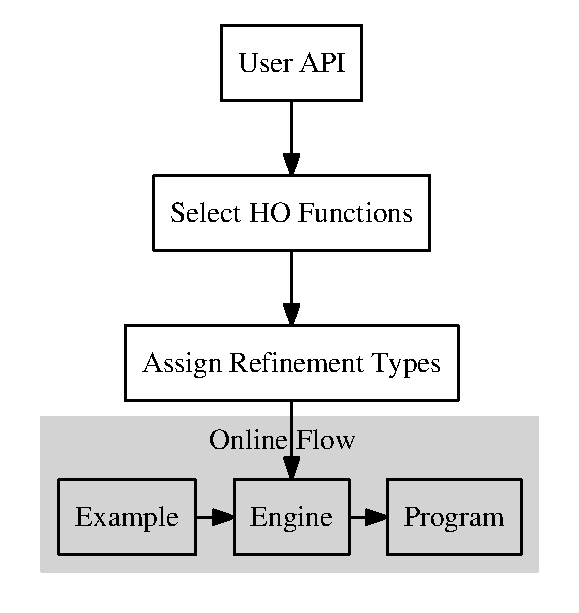
\includegraphics[width=0.45\textwidth]{algo}
  \caption{High-level structure of the algorithm.}
  \label{fig:high_level_overview}
\end{figure}

In this section, we give a high-level description of each component of our algorithm. Figure~\ref{fig:high_level_overview} below illustrates the ways in which these components interact. Broadly speaking, there are two main stages in the algorithm. The offline phase gathers the higher order declarations visible in the APIs and user-provided code, and assigns refinement types to them to build a custom synthesis \textit{engine}. This engine is then used during the online phase of the algorithm to search for functions that fit a set of supplied examples.

During the offline phase, the algorithm first scans the user-provided code, the libraries it imports, and the standard library to gather all of the functions and global values visible to the program. Then, it selects the higher-order functions from the set of all functions and values, and uses Liquid Haskell \cite{liquidhaskell} to assign refinement types to each one. Finally, each higher-order function is assigned a weight based on locality. User-defined functions are given the highest priority, while direct imports are given less, and the standard libraries are given the least. Together with the first-order functions and values, these triples of higher-order functions with their refinement types and weights are collected to produce a synthesis engine.

Once this stage is complete, the user can make online queries to the synthesis engine, which will search the space of constructable functions for those that fit the input examples. First, the engine computes a refinement type that fits the examples. This type is matched against the refinement types of the known higher-order functions, and the weights of each known function are adjusted based on how close the types match, if at all.

Once the candidate higher order functions have been chosen, the synthesis engine performs a best-first search for a program that fits all of the input and output examples by composing the candidates with first-order functions. For example, the higher-order function \texttt{map} might be supplied the \texttt{length} function if the example inputs are lists of lists of integers and the output examples are all lists of integers. The programs that are examined during the search are evaluated against the example set and are reported to the user as they match. Because the weights favor local declarations, the highest-ranked programs are likely to be the most idiomatic.

\subsection{Offline: Synthesis Engine Construction}
\subsection{Refinement type inference}

%>  filter ishigherOrder tys
We first collect all of the type signatures from our sources (user code, imports, and standard library). We filter through these to select only the higher order functions. Because in Haskell the function type constructor (->) is right binding, any higher order functions must have parenthesis in the type signature, which provides a convenient filtering predicate.

%> let uHOTyps = f 3000 typSigs
%> let iHOTyps = f 2000 importSigs
%> let pHOTyps = f 1000 preludeTypSigs
In order to rank the higher-order functions we assign weights based on their source location. User-defined functions are given the highest priority, while direct imports are given less, and the standard libraries are given the least. These rankings will contribute to the final ranking of candidate functions in the synthesis stage when we match the component function signatures on the examples.


%> hoRTyps <- mapM (addRType fc) (map fst allHOTyps)
%> HigherOrderFxn -> (injectRFxnType fxn .fst)
We automatically generate search space pruning hypotheses for our higher order functions.
In the case that the input and output types of the higher order functions are the same, we generate a LiquidHaskell predicate that relates the size of those types.
In this case, the hypothesis that applies to the higher order functions must also apply to the examples in order to consider that function as a candidate.
In the case that the input and output type are different, we defer the analysis to the synthesis stage and use our ranking system to good effect.

In order to derive these hypotheses, we require all higher order functions be be of a unified Kind (?) \texttt{$\_ \to * \to *$}, where the penultimate kind of the signature is the input and the final kind is the the output. functionally, this means we require that the user partially uncurry any higher order function they are interested in using during synthesis.

This is a simple procedure, but requires user knowledge of which parameters to the function will be given by the examples. 
As an example consider \texttt{zipWith' f (xs,ys) = zipWith f xs ys}, which will yield the type \texttt{zipWith' :: (a$\to$ b $\to$ c) $\to$ ([a],[b]) $\to$ [c]}. 
%The liquidHaskell predicate applied to this signature will be of the effect of \texttt{len([a],[b]) = len([c])}.


%> map rTypeTemplate ["=","<=",">="]
When the input and output types are the same, or use the same top level type constructor, we generate hypotheses as liquidHaskell predicates.
Our predicates specify size constraints on input and output of $\leq,\geq,=$.
For every predicate provided, we are able to more accurately prune the search space of higher-order functions, but we must test every higher-order function in scope on these predicates. 
Therefor, it is best to only select as many refinement types as is needed.
Although this offline stage only needs to be run once given a set of code and imports, liquidHaskell type checking is still fairly expensive.



\subsection{User defined data types}
%We focus only higher order functions that manipulate data structures
In order to support user defined data structures, we only require that a user implements some kind of measure\cite{realWorldLiquid} over their data structure.
This size function will help the system determine size constraints on the examples, so that we can pick higher order functions that might actually work.
In fact, a size function could just be a constant function, which means the system will test every higher-order function that fits the types. 
Maybe this should even be a builtin default?

As an example, take the code from section \ref{examples} for synthesizing a music function.
the user would have needed to provide a measure function for Music a.
This measure will allow liquidHaskell to draw conclusions about the size of examples of type [Music a :$\to$ Music a], as well as conclusions about higher order functions over the Music data structure.

\begin{minted}[fontsize=\footnotesize]{haskell}
import Euterpea

{-@ measure len @-}
len :: Music a -> Int
len m =
  case m of
    Prim _  -> 1
    m1 :+: m2 -> len m1 + len m2
    m1 :=: m2 -> len m1 + len m2
    Modify c m -> len m
\end{minted}


\subsection{Extending Liquid Haskell
}%this hasn't happened yet (and probably wont for this paper)
LiquidHaskell does not support certain popular syntax extensions to Haskell, such as LambdaCase (TODO list others). In the spirit of this work, we wish to support as much user defined code as possible. To this end, we can extend the refinement type system by allowing refinement type inference on repersentative examples of a higher order function. Take the following code (pick something from an actual library on hackage.

\begin{minted}[fontsize=\footnotesize]{haskell}
{-# LANGAUGE LambdaCase #-}

fooMap :: (a -> b) -> [a] -> [b]
fooMap f = \case
  [] -> []
  l -> map f l
 \end{minted}


We generate and applying many examples with QuickCheck for each higher order function.
We then apply a similar refinement type inference strategy as above to these examples.
This lets us support a larger subset of the language, and, in theory refinement type inference for other languages too!

There are however repercussions to this approach. We are not guaranteed to generate a correct refinement type because we might not generate a fully representative examples. So
\end{comment}

\subsection{Online: Fitting Functions to Examples}
Once the synthesis engine has been constructed, the system is ready to answer function fitting queries. When examples are provided, the synthesis engine finds a suitable refinement type for a hypothetical function that could fit that example. Then, this refinement type is matched via builtin type-checking against the higher order functions known to the engine.

Once the candidate functions are identified, a best-first search is initiated over combinations of the higher-order functions curried with each component function so that the combination type-checks. Each of these is executed against the set of inputs. Whenever a function produces the correct outputs for each input, it is said to fit, and is reported to the user. This search continues until the space is exhausted or it is manually interrupted.

As in section \ref{HORtypeInf}, we also consider two cases for examples. The first where the example input and output types match up to the top level type constructor, and the the case where the types do not match.

In the case that the types do match, we find the set of refinement types that the examples satisfy. Generating refinement type predicates about the size of the input and output, as in section \ref{HORTypes}, we run type inference on the input / output examples to \markk{the following is wrong, what is a basic rtype anyway?} get a basic refinement type. Then, the input-output pairs are matched against a fixed set of predicates to enrich the refinement type. These predicates could impose constraints such as the input list being of equal, lesser, or greater size to the output list. \markk{end things being junk} For instance, the example set:

\begin{lstlisting}
exs = [[1,2,3,4] :-> [1,3],
       [2,4,6,8] :-> [],
       [5,7] :-> [5,7]]
\end{lstlisting}

\noindent would have an inferred base type \markk{this isn't inferend right now, if we want to do that we would be using ghc, not LiqHask. check http://stackoverflow.com/questions/8963488/automatically-add-type-signatures-to-top-level-functions for a script to test} of \texttt{[Int] -> [Int]} and its final refinement type would be \texttt{xs:[Int] -> \{ ys:[Int] | len xs >= len ys \}}, since all of the examples suggest that the output list does not grow. The addition of these refinement type predicates dramatically reduces the search space in practice.

Once these higher order functions have been culled from the pool of candidates, we iterate through each in best-first order. For each higher-order function, we supply it with arguments until it is compatible with the type signature implied by the example set. By convention, we take the final argument of the function to be the input, which means that higher-order functions that take multiple inputs have to explicitly be uncurried. Value types are satisfied by selecting from a pool of default values, and function types are satisfied by searching for first-order functions that would make the resulting signatures match. If it is not possible to find values that fit, the search moves on to the next higher-order function.

\subsubsection{Dismantling procedure}

A \textit{dismantling procedure} prunes the first order function search space by using information from the top level examples, and the current state of synthesis.
Any particular instance of deductive of reasoning can be applied to dismantle top level information.
From the specific examples, we might deduce constraints on the component function.
Given a candidate higher order function, we can also infer type constraints on the component function.
In either case, we use abductive reasoning to make a guess at the function, which then guide our further search.

We specialize the type of the higher order function to the examples as much as possible.
Since examples must be given as a concrete type, we can always specialize a our candidate higher order function. 

\begin{lstlisting}
specializeOn :: Type -> Type -> Type
specializeOn concTy hoTy =
  replaceTysIn hoTy typeMap
  where
    typeMap = makeTypeMap 
                concTy 
                (lastAsFunType hoTy)
                Map.empty
\end{lstlisting}

Given this partially concrete type for the higher order function, we search for first order functions that will fit the component signature.
If the component signature is a concrete instance of the first order function, we can also accept it as a possibility.
This occurs when we try to use \texttt{id::a->a} as a component for \texttt{::Int->Int}.

Note that at this stage of synthesis, we can never have a first order function that is a concrete instance of the component signature. 
An example of this would be trying to use \texttt{negate::Int$\to$Int} as a component for \texttt{::a$\to$a}
Given our requirement that all type variables are determined by the uncurried input from section \ref{exampleSyntax}, we will have specialized all type variables with the \texttt{specializeOn} function.
That means the component function must be concrete at this stage.
This is really good for performance.


In the case that neither of those situations hold, we try to apply a value to the first order function.
For instance, if the component signature is \texttt{::Int->Int}, and we have the first order functions \texttt{(+)::Int->Int->Int}, we apply some initial values to \texttt{(+)} to get a new function (e.g. \texttt{(+1)}) that fits the component signature.

If the initial value's type is an instance of Monoid, we can extract the unit value (named mempty in Haskell's monoid typeclass\cite{}) to use as our initial value. For lists, the unit element is []. However, there are two valid monoids for numbers, using either (+) or (*) as the operators and resulting in unit elements 0 and 1 respectively. We take both of these values (along with other useful values of -1, 2, and 3) as possibilities since the cost of testing both values is relatively small.

However, requiring our users to write monoid instances for their datatypes may be a nuisance. Additionally, users may have some domain knowledge that a particular value may be useful in their application. Since our system automatically considers functions defined in the user code base, users may simply write their own specializations of the higher order functions, or provide useful initial values, to be used in synthesis. 

\begin{lstlisting}
-- to use 5 as an initial value for foldl
foldl :: (a -> b -> a) -> [b] -> a
foldl5 f i o = foldl f 5 i o

-- to use 5 as an initial value in all recursions
initVal :: Int
initval5 = 5
\end{lstlisting}


In the implementation, we actually build new functions with the name of the composed functions, and adjust the type signature accordingly.



%If the types of a higher order function do not match, we 



To choose the component function we weighted subtyping algorithm.
When two types have weight of >1, we will say type a \textit{generalizes} type b.
\markk{someone probably wrote something about this, just need to find out where and cite.}
If we have the higher order function map :: (a$\to$b) $\to$ [a] $\to$ [b] and the examples :: [Int] $\to$ [Int], then our component function f might have f::a$\to$b, or f::Int$\to$Int, or f::Int$\to$a, but certainly not f::[Bool]$\to$[Bool].

The cost relation can be formalized as follows in the pseudocode for the cost function function c.
\begin{lstlisting}

c :: Type -> Type -> Maybe Int
c (TyParen t1) (TyParen t2) =
  fmap (1+)  c t1 t2
c (TyFun t1 t1') (TyFun t2 t2') =
   fmap (1+) (liftA2 (+) (c t1 t2) (c t1' t2'))
c (TyCon q1) (TyCon q2) =
   if (q1==q2) then Just 20 else Nothing
c \_ \_ = Nothing

\end{lstlisting}

This cost function is used below.

We identify two separate classes of higher order functions - those that take a single first order function, and those that need initial values in addition to a function. The \texttt{map} function only takes a first order function, while \texttt{foldl :: $(a\to b\to a)\to a\to [b]\to a$} requires an initial value for \texttt{a}. While the process described so far handles the former, initial values must also be addressed.

To identify initial values in a type signature, we can use our previous assumption that all higher order function have been partially curried to the type \texttt{$\_\to *\to*$}. Adding the further assumption that only one first order function maybe be passed to the higher order function, we simply tag any non-function type in the hole as an initial value. 



\section{Evaluation}
\subsection{Optimizations}

Since the standard library can be considered a relatively stable set of code, we can cache the refinement type inference to reduce the build time.
On my machine, it removes ~40 seconds from the build time.

\section{Related Work and Conclusions}\label{conclusions}
\subsection{Limitations}

Without subexample generation we cannot recursively apply our algorithm to create programs with multiple applications of higher order functions as in the   $\Lambda^2$ paper\cite{isil}. Since they provide hard coded subexample generation hypotheses for the higher order functions they use, this does not scale.

With the eventual goal of building a complete program synthesis engine, we will need to integrate the first order function synthesis. While this problem has been investigated in isolation, it is not clear how to efficiently determine if  a set of examples will require a higher order function or a first order function.

\bibliographystyle{abbrvnat}
\bibliography{sample}

\end{document}
